\section{Reference Frames}
\label{reference_frames}


In this section we will review four commonly used reference frames that are
used in order to localize a rigid body. 

\subsection{Earth-Centered Inertial Frame or ECIF}

The first frame is the Earth-Centered
Inertial Frame or ECIF. This frame has its origin
at the center of the earth, the $z$ axis points true north, and the $x$ and $y$ axis are fixed with
respect to the very distant stars. This means that although the earth
rotates about the $z$ axis, the $x$ and $y$ axes do not move. 

\begin{figure}[!htb]
\begin{center}
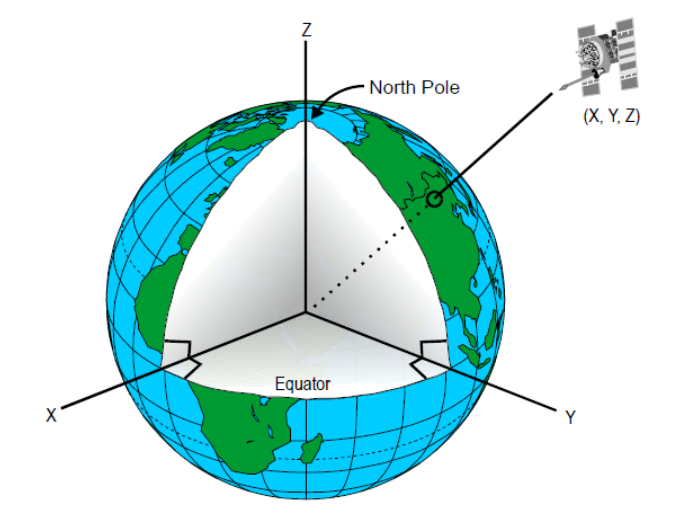
\includegraphics[scale=0.290]{img/coordinate_transforms/ref_frame_1.jpeg}
\end{center}
\caption{Schematic of ECIF.}
\label{ref_frame_1}
\end{figure}

\subsection{Earth-Eentered Earth-Fixed Frame, or ECEF}

Next, the Earth-Eentered Earth-Fixed Frame, or ECEF is just like ECIF except that its $x$ axis is aligned with the Prime
Meridian and spins with the earth. The $y$ axis is determined
by the right-hand rule. 

\begin{figure}[!htb]
\begin{center}
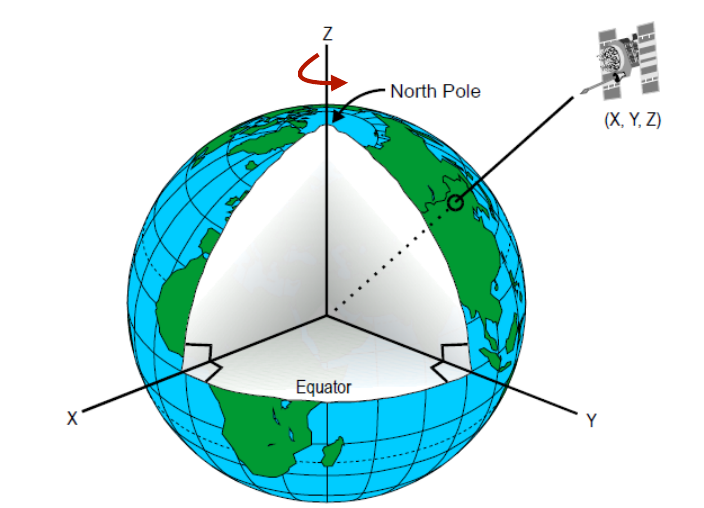
\includegraphics[scale=0.290]{img/coordinate_transforms/ref_frame_2.jpeg}
\end{center}
\caption{Schematic of ECEF.}
\label{ref_frame_2}
\end{figure}


The difference between the ECEF and ECIF is that the former is fixed to the earth, while the ECIF,  is fixed with
respect to the distance stars. 


\subsection{North East Down or NED}

Although ECEF and ECIF are useful when we discuss satellites and
inertial sensing onboard aircraft, for practical car applications, we will usually want to use a frame that
is fixed with respect to the ground. For this, we will use what we referred
to as the navigation frame. A very common navigation frame
is one that is attached to some germane starting point and
aligned with north, east, and down abbreviated as NED. Figure \ref{ref_frame_3} shows schematically the NED frame

\begin{figure}[!htb]
\begin{center}
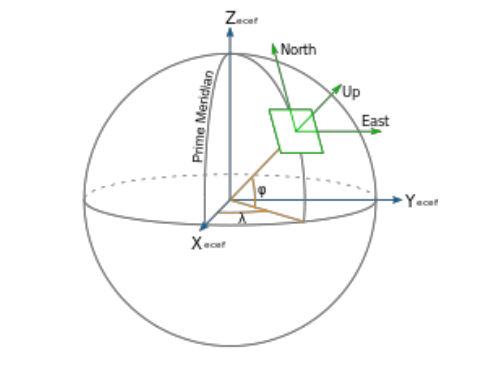
\includegraphics[scale=0.290]{img/coordinate_transforms/ref_frame_3.jpeg}
\end{center}
\caption{Schematic of NED.}
\label{ref_frame_3}
\end{figure}


\subsection{Body and sensor frames}

Often, we also need to think about a sensor frame that is rigidly
attached to a sensor like a LiDAR, a GPS receiver, or
an inertial measurement unit. This frame will typically be distinct
from the general vehicle frame, which can be placed anywhere on
the vehicle that is convenient, at the center of mass for example. For localization, we will often
ignore the distinction between the vehicle and sensor frame and assume
that if we can track the sensor, we should be able to track any point on the vehicle given proper calibration. 

